\begin{wrapfigure}{r}{0.5\textwidth}
% \vspace{-10pt}
\resizebox{0.48\textwidth}{!}{
        \tablestyle{7pt}{1.05}
        \begin{tabular}{y{55}x{43}x{22}x{30}}
            Algorithm & \modela{A}$\leftrightarrow$\modela{A}/\modelb{B}$\leftrightarrow$\modelb{B}? & Acc & Time\\
            \shline
            Identity {\scriptsize (Eq.~\ref{eq:wavg})}                  & \xmark{} & {43.0\conf{3.1}} & {1.8\unit{ms}} \\
            Permute {\scriptsize (Eq.~\ref{eq:rebasin})}                & \xmark{} & {58.4\conf{1.3}} & {28\unit{ms}} \\
            K-Means                                                     & \checkmark{} & {29.1\conf{5.5}} & {19\unit{sec}} \\
            \hline
            \multicolumn{4}{c}{Zip {\scriptsize (Eq.~\ref{eq:zip})}} \\
            Optimal Match                                               & \checkmark{} & {\bf 79.6\conf{1.7}} & {11\unit{min}} \\
            Greedy Match                                                & \checkmark{} & {\bf 79.0\conf{1.8}} & {1.1\unit{sec}} \\
            Greedy, $\alpha$=0.1 & \default{\checkmark{}} & \default{\textbf{79.1\conf{2.1}}}  &  \default{1.2\unit{sec}}  \\
        \end{tabular}
    }
    \captionof{table}{{\bf Comparing Matching Algorithms} to use for \modelc{$M_i$} on CIFAR-10 (5+5) joint 10-way accuracy.
    Permuting \modelb{B}$\rightarrow$\modela{A} as in prior work (Eq.~\ref{eq:rebasin}) performs poorly. 
    We significantly improve by merging features \textit{within} each model (Eq.~\ref{eq:zip}).
    Our greedy approach is nearly as accurate as the optimal algorithm while being two orders of magnitude faster. 
    }
    \label{tab:matching_alg}
    \vspace{-10pt}
\end{wrapfigure}
% \end{table}


% \begin{wrapfigure}{l}{0.48\linewidth}
% % \vspace{-260pt}
% \begin{minipage}[l]{\linewidth}{
%     \begin{minipage}[c]{\linewidth}
%         \centering
%         \resizebox{\textwidth}{!}{
%             \tablestyle{7pt}{1.05}
%             \begin{tabular}{y{55}x{43}x{22}x{30}}
%                 Algorithm & \modela{A}$\leftrightarrow$\modela{A}/\modelb{B}$\leftrightarrow$\modelb{B}? & Acc & Time\\
%                 \shline
%                 Identity {\scriptsize (Eq.~\ref{eq:wavg})}                  & \xmark{} & {43.0\conf{3.1}} & {1.8\unit{ms}} \\
%                 Permute {\scriptsize (Eq.~\ref{eq:rebasin})}                & \xmark{} & {58.4\conf{1.3}} & {28\unit{ms}} \\
%                 K-Means                                                     & \checkmark{} & {29.1\conf{5.5}} & {19\unit{sec}} \\
%                 \hline
%                 \multicolumn{4}{c}{Zip {\scriptsize (Eq.~\ref{eq:zip})}} \\
%                 Optimal Match                                               & \checkmark{} & {\bf 79.6\conf{1.7}} & {11\unit{min}} \\
%                 Greedy Match                                                & \checkmark{} & {\bf 79.0\conf{1.8}} & {1.1\unit{sec}} \\
%                 Greedy, $\alpha$=0.1 & \default{\checkmark{}} & \default{\textbf{79.1\conf{2.1}}}  &  \default{1.2\unit{sec}}  \\
%             \end{tabular}
%         }
%         \captionof{table}{{\bf Matching Algorithm} to use for \modelc{$M_i$}. 
%         Permuting \modelb{B}$\rightarrow$\modela{A} as in prior work (Eq.~\ref{eq:rebasin}) performs poorly, thus we allow merging features \textit{within} each model (Eq.~\ref{eq:zip}).
%         Our greedy approach is nearly as accurate as the optimal algorithm while being two orders of magnitude faster. 
%         ``Acc'' is CIFAR-10 (5+5) joint 10-way accuracy.
%         }
%         \label{tab:matching_alg}
%     \end{minipage}
%     \vspace{10pt}
%     \begin{minipage}[c]{\linewidth}
%         % \vspace{40pt}
%         \centering
%         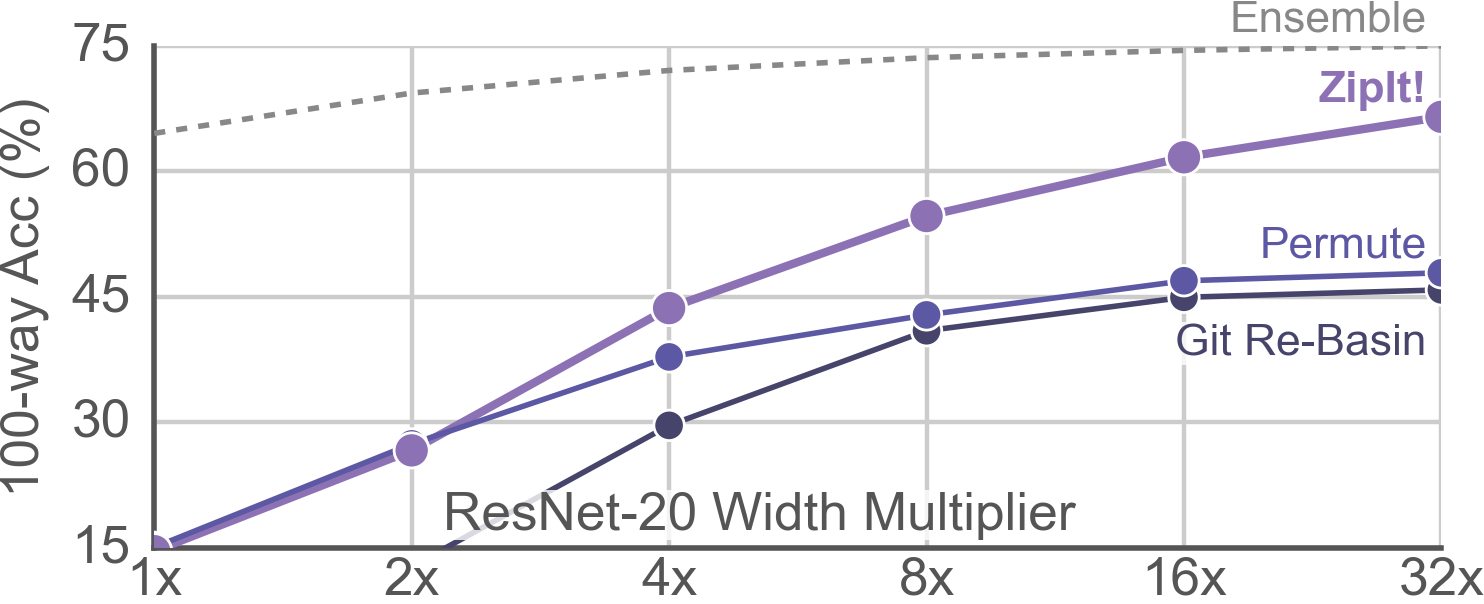
\includegraphics[width=0.95\linewidth]{figures/imgs/model_scale.png}
%         \caption{{\bf Model Scale.} 
%         \name{}\ makes effective use of extra model capacity to quickly reach the ensemble on CIFAR-100 (50+50) when we increase the width of ResNet-20 models.
%         % \name{}\ quickly approaches ensemble accuracy as we increase the width of the ResNet-20 models in the CIFAR-100 (50+50) setting, making effective use of extra capacity from scale.
%         % As we increase the width of the ResNet-20 models used for the CIFAR-100 (50+50) setting, \name{}\ makes effective use of that extra capacity, quickly approaching ensemble accuracy. 
%         Git Re-Basin \cite{ainsworth2022git} and Permute only slightly benefit from the extra scale.
%         }
%         \label{fig:model_size}
%         \vspace{-30pt}
%     \end{minipage}
% }\end{minipage}
% \end{wrapfigure}










% \begin{table}[t]
% \centering

% \tablestyle{7pt}{1.05}
% \begin{tabular}{y{50}x{43}x{22}x{30}}
%     Algorithm & \modela{A}$\leftrightarrow$\modela{A}/\modelb{B}$\leftrightarrow$\modelb{B}? & Acc & Time\\
%     \shline
%     Identity {\scriptsize (Eq.~\ref{eq:wavg})}                  & \xmark{} & {43.0\conf{3.1}} & {1.8\unit{ms}} \\
%     Permute {\scriptsize (Eq.~\ref{eq:rebasin})}                & \xmark{} & {58.4\conf{1.3}} & {28\unit{ms}} \\
%     K-Means                                                     & \checkmark{} & {29.1\conf{5.5}} & {19\unit{sec}} \\
%     \hline
%     \multicolumn{4}{c}{Zip {\scriptsize (Eq.~\ref{eq:zip})}} \\
%     Optimal Match                                               & \checkmark{} & {\bf 79.6\conf{1.7}} & {11\unit{min}} \\
%     Greedy Match                                                & \checkmark{} & {\bf 79.0\conf{1.8}} & {1.1\unit{sec}} \\
%     Greedy, $\alpha$=0.1 & \default{\checkmark{}} & \default{\textbf{79.1\conf{2.1}}}  &  \default{1.2\unit{sec}}  \\
% \end{tabular}
% \caption{{\bf Matching Algorithm} to use for \modelc{$M_i$}. 
% Permuting \modelb{B}$\rightarrow$\modela{A} as in prior work (Eq.~\ref{eq:rebasin}) performs poorly, thus we allow merging features \textit{within} each model (Eq.~\ref{eq:zip}).
% Our greedy approach is nearly as accurate as the optimal algorithm while being two orders of magnitude faster. 
% ``Acc'' is CIFAR-10 (5+5) joint 10-way accuracy.
% }
% \label{tab:matching_alg}
% \end{table}
